\documentclass{scrartcl}

\usepackage{url}

\usepackage{graphicx}
\usepackage{subfig}
\usepackage{tikz}
    \usetikzlibrary{calc, arrows, positioning, shapes.geometric}
\usepackage{pgfplots}
    \pgfplotsset{compat=1.8}
    \usepgfplotslibrary{groupplots}
\usepackage{multirow}
\usepackage{booktabs}
\usepackage{xspace}

\usepackage{hyperref}
    \hypersetup{colorlinks=true, allcolors=black}
\usepackage[noabbrev, nameinlink]{cleveref}

\usepackage[textsize=footnotesize,color=white,bordercolor=red,linecolor=red]{todonotes}
\let\newtodo\todo
% define your own comment environment if you like:
\newcommand{\patrick}[1]{\newtodo[inline]{\color{magenta}Patrick says ``#1''}}

\newcommand{\baxterdotnet}{Baxter.NET\xspace}
\newcommand{\baxterrpc}{Baxter RPC\xspace}

\title{SmartFactories Baxter Anomaly Data Set}
%\subtitle{Where are we and where do we go from here}
\author{Marvin Ludersdorfer\\\texttt{ludersdorfer@fortiss.org}}
\date{\today}

\begin{document}
\maketitle

\begin{abstract}
    \em
    Anomaly detection is an important task in the control of (industrial) robots.
    We select generic robot motion as our problem to do anomaly detection on since this is part of and covers a wide range of robot tasks.
    Our approach is to apply various machine learning algorithms to the problem of anomaly detection in robot motion.
    To this end, the first step is to record an appropriate data set to work with.
    
    In this article, we first explain the reasoning that motivated the Baxter anomaly data set.
    We then describe the framework we implemented to record the data set.
    After discussing the structure of the data set, we conclude by presenting some preliminary analysis of the data and intuitions useful for interpreting these.
\end{abstract}

\tableofcontents

\section{Introduction}
    Consider the very typical usecase of a pick-and-place task performed with an industrial robot.
    For the sake of the argument, let the robot be located next to, say, an injection molding machine that is producing plastic parts for the interior of a particular production series of cars of some renowned automobile manufacturer.
    The machine closes the mold, molten plastic is injected into the mold, and once the thermoplastic or duroplast material is cooled down sufficiently, the machine opens the mold.
    Now the robot moves its end-effector into the machine, picks up the freshly produced part, takes it out of the machine and places it on a conveyor belt which takes the parts to some post-production step like quality inspection or packaging.
    Simultaneously the machine closes the mold again and the cycle starts anew.\footnote{Note that we could have taken the example of almost any other application of robots in an industrial environment---such as welding or painting---and still would come to the same conclusion as we will with this illustrative example.}
    
    From the above example we choose the important subtask of robot motion for the development of anomaly detection algorithms.
    This is because failures in the process of grasping or releasing the object (ignoring the appropriate positioning of the end-effector in case poses are not ``teached in'' manually) can be detected fairly easily (e.g. gripper position or -force for mechanical grippers, or pressure if vacuum grippers are used).

\section{Definition of Anomalies}
    For this data set, we restrict anomalies in robot motion to correspond to a change in the dynamic behavior of the robot.
    In this sense we are able to model anomalies by modifying the robot's control parameters.
    
    That is, for the experiment we construct the following framework.
    The industrial robot in the example above is instantiated as a Baxter Research Robot\footnote{See \url{http://www.rethinkrobotics.com/baxter-research-robot/} for more information.}.
    Furthermore, the injection molding machine and conveyor belt are abstracted away and the process of picking up a part from within the machine and placing it on the conveyor belt is represented by the Baxter robot moving between configurations sampled at random from the workspace of the robot.
    
    \subsection{Definition of Feasible Workspace}
    \label{ssec:workspace}
        We define the feasible workspace for this experiment by defining twelve corners of a three-dimensional space we consider the Baxter robot to be able to reach with its end-effector, as illustrated in \cref{fig:baxterws}.
        \begin{figure}
            \centering
            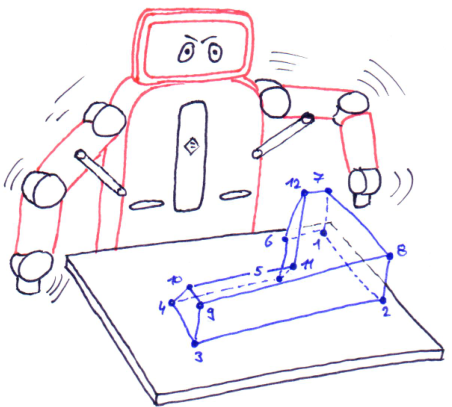
\includegraphics[width=0.45\textwidth]{figs/baxterws}
            \caption{Definition of feasible workspace by means of definition of twelve corners of a three-dimensional space reachable by the Baxter robot.
                Here illustrated for the left arm.}
            \label{fig:baxterws}
        \end{figure}
        To this end, we use the method \verb|ReadPoseAngles(12)| from our \baxterdotnet framework (see \cref{sec:baxterdotnet}) to manually and consecutively locate Baxter's left arm in each of the twelve configurations and record the corresponding Cartesian poses as well as---via the robot's inverse kinematics---a valid joint angle configuration for each of the poses.
        
        Since drawing random samples from the three-dimensional workspace is no trivial task, we devise the following procedure.
        The recorded poses are read in MATLAB and the convex hull of the twelve positions ($x$-, $y$-, $z$-components of the poses) is computed.
        Let this convex hull be called the feasible workspace hereafter.
        We now compute $200$ pseudo-uniform Latin hypercube\footnote{Latin hypercube sampling is a statistical method for generating samples from a  multidimensional distribution, where each sample is the only one in each axis-aligned hyperplane containing it. See \url{https://en.wikipedia.org/wiki/Latin_hypercube_sampling}.} samples, transform the unit cube in the range of the convex hull, and find those samples that lie inside the feasible workspace.
        This is done by running the MATLAB script \verb|poses.m| and gives $63$ valid positions as illustrated in \cref{fig:poses}.
        \begin{figure}
            \centering
            \begin{tikzpicture}
                \begin{groupplot}[
                    group style={
                        group size=3 by 1, 
                        horizontal sep=3\baselineskip
                    },
                    scale only axis,
                    width=.25\textwidth,
                    scatter/classes={c={mark=o, draw=blue}, s={mark=x, draw=green}}
                    ]
                    \nextgroupplot[height=.25\textwidth, title={$xy$-plane}]
                    \addplot[scatter, only marks, scatter src=explicit symbolic] table[x=x, y=y, meta=label]{figs/poses.dat};
                    \nextgroupplot[height=.25\textwidth, title={$yz$-plane}]
                    \addplot[scatter, only marks, scatter src=explicit symbolic] table[x=y, y=z, meta=label]{figs/poses.dat};
                    \nextgroupplot[height=.25\textwidth, title={$xz$-plane}]
                    \addplot[scatter, only marks, scatter src=explicit symbolic] table[x=x, y=z, meta=label]{figs/poses.dat};
                \end{groupplot}
            \end{tikzpicture}
            \caption{Visualization of $63$ pseudo-uniform positions in the feasible workspace of Baxter's left arm.
                Blue circles represent the twelve corners of the workspace.
                Green crosses represent the $63$ pseudo-uniform valid samples.
                Note that the samples are distributed sufficiently uniform in the feasible workspace.}
            \label{fig:poses}
        \end{figure}
        Without loss of generality we use a constant desired orientation for the end-effector to obtain $63$ valid poses in the feasible workspace of Baxter's left arm.
        These are saved to a file and stored for later use in the experiment.
        
    \subsection{Description of Experiment}
    \label{ssec:experiment}
        As stated before, the experiment consists of the Baxter robot repeatedly moving its left arm ($N$ trials) between a number of pseudo-randomly sampled poses ($p$ poses) in the feasible workspace.
        The $p$ poses and the order in which the robot moves through them is kept fixed between the $N$ trials.
        The procedure of the experiment is described in the following and illustrated in \cref{fig:experiment}.
        \begin{figure}
            \centering
            \footnotesize
            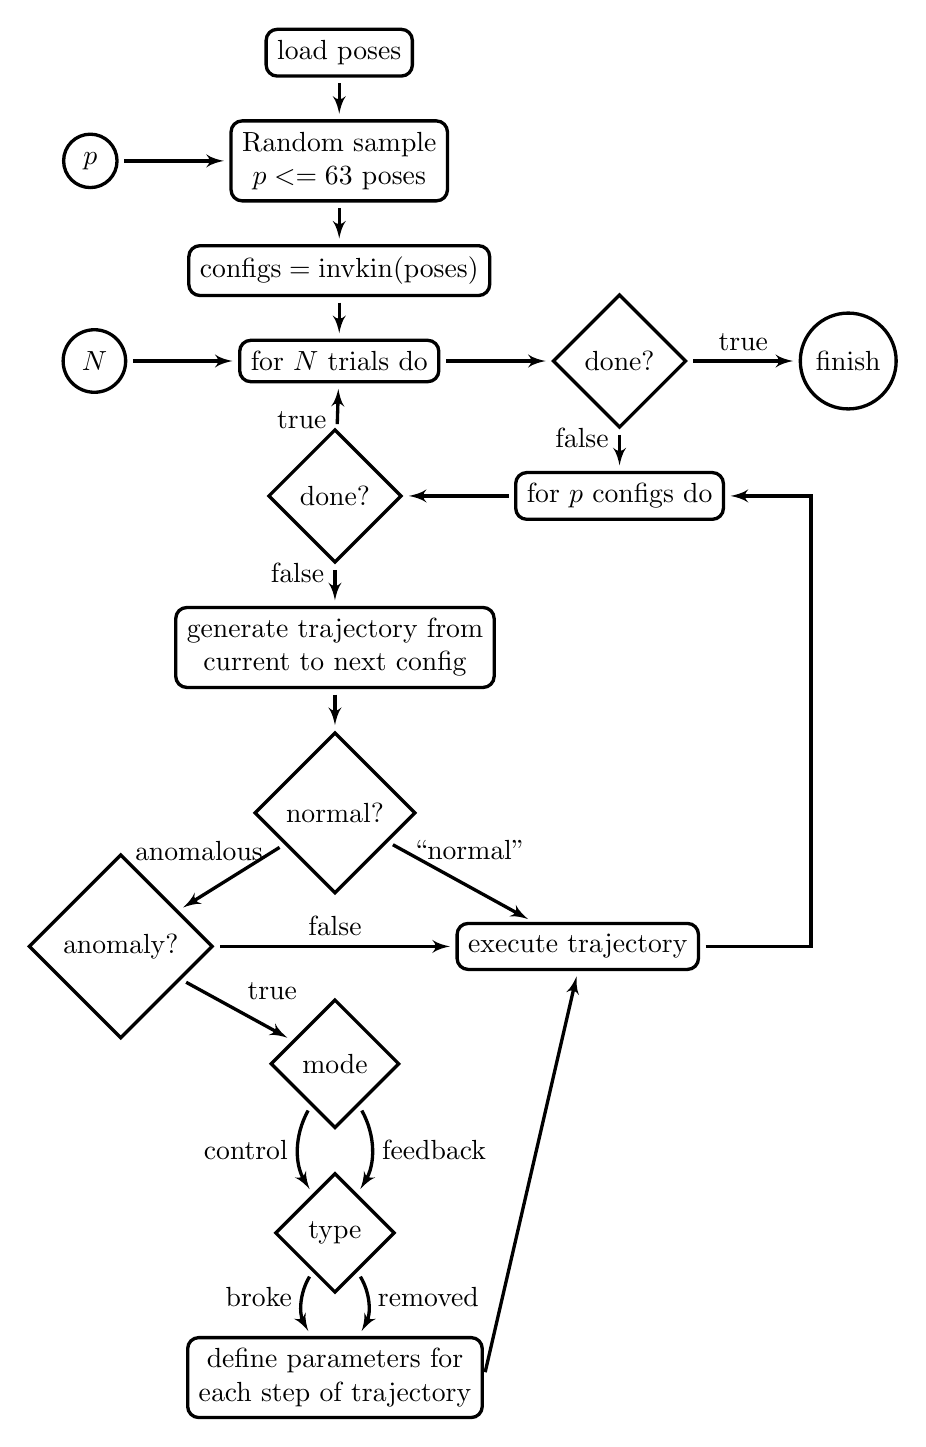
\begin{tikzpicture}[node distance=15pt and 40pt, auto,
                block/.style = {
                    rectangle, rounded corners,
                    draw=black,
                    very thick, inner sep=.4em,
                    minimum size=1em, text centered,
                    align=center
                },
                inpt/.style = {
                    circle,
                    draw=black,
                    very thick, inner sep=.4em,
                    minimum size=1em, text centered,
                    align=center
                },
                decision/.style = {
                    diamond,
                    draw=black,
                    very thick, inner sep=.4em,
                    minimum size=1em, text centered,
                    align=center
                },
                arrow/.style = {
                    draw, ->, >=latex', shorten >=2pt,
                    shorten <=2pt, very thick
                }
                ]
                
                \node[block] (load) {load poses};
                \node[block, below=of load] (samplep) {Random sample\\$p<=63$ poses};
                \node[inpt, left=of samplep] (p) {$p$};
                \node[block, below=of samplep] (invkin) {$\mathrm{configs}=\mathrm{invkin(poses)}$};

                \node[block, below=of invkin] (forN) {for $N$ trials do};
                \node[decision, right=of forN] (forNd) {done?};
                \node[inpt, left=of forN] (N) {$N$};
                \node[inpt, right=of forNd] (exit) {finish};

                \node[block, below=of forNd] (forp) {for $p$ configs do};
                \node[decision, left=of forp] (forpd) {done?};
                \node[block, below=of forpd] (gen) {generate trajectory from\\current to next config};
                \node[decision, below=of gen] (normal) {normal?};
                \node[draw=none, below=of normal] (b1) {};
                \node[decision, left=of b1] (samplea) {anomaly?};
                \node[decision, below=of b1] (mode) {mode};
                \node[block, right=of b1] (traj) {execute trajectory};
                \node[decision, below=of mode] (type) {type};
                \node[block, below=of type] (pars) {define parameters for\\each step of trajectory};
                \node[draw=none, right=of pars] (b2) {};
                \node[draw=none, right=of traj] (b3) {};


                \path[arrow] (load)--(samplep);
                \path[arrow] (p)--(samplep);
                \path[arrow] (samplep)--(invkin);
                \path[arrow] (invkin)--(forN);

                \path[arrow] (N)--(forN);
                \path[arrow] (forN)--(forNd);
                \path[arrow] (forNd) edge node[left, pos=0.2] {false} (forp);
                \path[arrow] (forNd) edge node[above] {true} (exit);

                \path[arrow] (forp)--(forpd);
                \path[arrow] (forpd) edge node[left, pos=0.2] {false} (gen);
                \path[arrow] (forpd) edge node[left, pos=0.2] {true} (forN);
                \path[arrow] (gen)--(normal);
                \path[arrow] (normal) edge node[right, pos=0.1] {``normal''} (traj);
                \path[arrow] (normal) edge node[left, pos=0.1] {anomalous} (samplea);
                \path[arrow] (samplea) edge node {false} (traj);
                \path[arrow] (samplea) edge node {true} (mode);
                \path[arrow] (mode) edge[bend right] node[left] {control} (type);
                \path[arrow] (mode) edge[bend left] node {feedback} (type);
                \path[arrow] (type) edge[bend right] node[left, pos=0.4] {broke} (pars);
                \path[arrow] (type) edge[bend left] node[right, pos=0.4] {removed} (pars);
                \path[arrow] (pars.east) -- (traj.south);
                \path[arrow] (traj.east)--(b3.west) |- (forp.east);
            \end{tikzpicture}
            \caption{Flow diagram of experiment.
                For a description see \cref{ssec:experiment}.}
            \label{fig:experiment}
        \end{figure}
    
        \subsubsection{Generation of ``Normal'' Data}
            ``Normal'' data---i.e., data that is supposedly free of anomalies---is generated by $N$ times moving through the $p$ poses sampled from the $63$ valid poses generated as described in \cref{ssec:workspace}.
    
        \subsubsection{Generation of Anomalous Data}
        \label{sssec:anomaly}
            Anomalous data is generated in the same manner as the ``normal'' data with the distinction that in each of the $N$ trials for each of the $p-1$ sub-movements between two consecutive poses, $p_{\mathrm{start}}$ and $p_{\mathrm{end}}$, with a probability of $\Pi$ an anomaly is introduced.
            As stated before, such an anomaly is generated by modifying the control parameters of the robot.
            This is achieved as follows (see \verb|Baxter.move_to_joint_positions_anomaly| in our \baxterrpc framework (\cref{sec:baxterrpc})).
            If an anomaly is due, one of the seven joints of Baxter's arm is chosen at random.
            A trajectory between $p_{\mathrm{start}}$ and $p_{\mathrm{end}}$ is computed on joint level.
            If the desired number of anomalous steps, $t_{a,\mathrm{des}}$, is larger than the number of steps in the trajectory, $t_{a,\mathrm{des}}$ is reduced accordingly.
            The step of the trajectory for the anomaly to start in is sampled at random from an appropriate interval.
            Depending on the type of anomaly selected (see \cref{tab:types}), either the P-component of the sampled joint's PID controller, $k_{P,j}$, is multiplied by a factor of $f$ or set to zero, or the feedback value, $s$, of the controller is biased with Gaussian noise or set to zero during the $t_{a,\mathrm{des}}$ steps of the trajectory that are selected to be anomalous.
            \begin{table}
                \centering
                \caption{Modes and types of anomalies implemented in the \baxterrpc and \baxterdotnet frameworks.}
                \label{tab:types}
                \begin{tabular}{lllp{5cm}}
                    \toprule
                    anomaly mode & anomaly type & parameter changed & description \\
                    \midrule
%                    manual & -- & -- & anomaly inflicted by manually hitting the robot \\ 
%                    \midrule
                    \multirow{3}{*}{control} & broken & $k_{P,j} \leftarrow k_{P,j}f$ & control parameter modified by multiplicative constant \\
                    & removed & $k_{P,j} \leftarrow 0$ & control parameter removed \\
                    \midrule
                    \multirow{3}{*}{feedback} & broken & $s \leftarrow s + \mathcal{N}(0, \varepsilon)$ & feedback modified by additive Gaussian noise \\
                     & removed & $s \leftarrow 0$ & feedback removed \\
                    \bottomrule
                \end{tabular}
            \end{table}
            After these steps are executed, the modified parameter is returned to its default value.

    \subsection{Peculiarities of Modifying Control Parameters}
        Since the control parameter in the Baxter SDK provided by Rethink Robotics are not accessible, we wrote our own controller for the robot arm motion.
        It makes use of the torque control mode provided by the Baxter SDK.
        The principle is as follows.
        Each of the seven joint angles of an arm is controlled by a dedicated, independent PID controller.
        That is, the desired and current joint angles are compared and the PID control law 
        \begin{equation}
        \label{eq:pid}
            \tau_t = k_P(q_{d,t} - q_t) + k_I\sum_{i=0}^t(q_{d,i} - q_i) - k_D\dot{q_t}
        \end{equation}
        is used to convert joint angle deviations to corresponding motor torques required to compensate for the offset.
        In (\ref{eq:pid}) index $t$ is the current time step (or step of the trajectory), $q, \dot{q}$ are the current joint angle and joint velocity, respectively, $q_d$ is the desired joint angle and $k_P, k_I, k_D$ are the P, I and D parameters of the joint controller.
        Finally, $\tau_t$ is the motor torque generated by the controller at step $t$.
        This PID controller is implemented in \verb|control/pid.py| in our \baxterrpc framework.
        
        Then, at each step of the trajectory, seven PID controllers have to be evaluated and their generated torques be commanded to the robot.
        This is what is described by \emph{execute trajectory} in \cref{fig:experiment} and implemented in \verb|Baxter.move_to_joint_positions| and \verb|Baxter.move_to_joint_positions_anomaly| in the \baxterrpc framework.
        Both functions are callable via \verb|baxterWrapper.Limb.PidMoveToJointPositions| from our \baxterdotnet framework.
    
\section{Description of Data Set}
    The procedure described in the previous section was used to record two data sets of $N=100$ trials each; one without anomalous data and one with the control parameter, $k_{P,i}$, being multiplied by a factor of $f=10$ if an anomaly was sampled with $\Pi = 0.5$.\patrick{0.5 is way to large!}
    In order to be able to compare both data sets the $p=10$ poses for the experiments were kept fixed.
    In particular, we used the poses 50, 47, 26, 27, 9, 61, 13, 55, 15 and 37 from the recorded set of 63 valid poses (see \cref{ssec:workspace}).
    
    \subsection{Data Recording}
        The data was recorded by running the \verb|dataAcquisition|-Program from our \baxterdotnet framework with the command line arguments summarized in \cref{tab:args}.
        This program implements the procedure described in \cref{ssec:experiment}.
        \begin{table}
            \centering
            \caption{Command line arguments used for recording the anomaly-free and anomalous data.}
            \label{tab:args}
            \begin{tabular}{lllllll}
                \toprule
                \multirow{2}{*}{Experiment} & \multicolumn{6}{c}{command line arguments} \\ \cline{2-7}
                & arm & trials & anomalies & mode & type & csv \\
                \midrule
                ``normal'' & left & 100 & false & 1 (control) & 0 (broken) & poses2.txt \\
                anomalous & left & 100 & true & 1 (control) & 0 (broken) & poses2.txt \\
                \bottomrule
            \end{tabular}
        \end{table}
        The following information was recorded:
        \begin{itemize}
            \item measured wrist acceleration: (timestamp, x, y, z)
            \item commanded configuration: (timestamp, s0, s1, e0, e1, w0, w1, w2)
            \item measured configuration: (timestamp, s0, s1, e0, e1, w0, w1, w2)
            \item generated torques: (timestamp, s0, s1, e0, e1, w0, w1, w2)
            \item commanded torques: (timestamp, s0, s1, e0, e1, w0, w1, w2)
            \item measured torques: (timestamp, s0, s1, e0, e1, w0, w1, w2)
            \item camera images: timestamp, flattened pixel vector
        \end{itemize}
        The indices s0, s1, e0, e1, w0, w1 and w2 identify joints of Baxter's arms as defined in \cref{fig:baxterjoints}.
        \begin{figure}
            \centering
            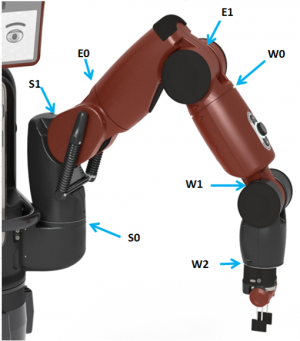
\includegraphics[width=.3\textwidth]{figs/baxterjoints}
            \caption{Definition of joint names.}
            \label{fig:baxterjoints}
        \end{figure}
        Images are recorded at a resolution of $320\times 200$ pixels.
    
    \subsection{Structure of the Data Set}
        The ``normal'' data is stored in \texttt{201508061628without.h5}, the data with anomalies in \texttt{201508071533with.h5}.
        Both files share the same structure as described in the following.
        Each data file contains 100 trials ($0, \ldots, 99$).
        Each trial in turn contains four groups, namely acceleration, configuration, effort and images.
        These groups are defined as follows (also see \cref{fig:h5}).
        \begin{figure}
            \centering
            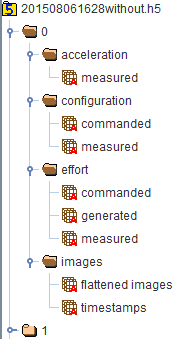
\includegraphics[width=.2\textwidth]{figs/h5}
            \caption{The structure of the recorded data sets.}
            \label{fig:h5}
        \end{figure}
        Acceleration contains one data field, measured.
        Configuration contains two data fields, commanded and measured.
        Effort contains three data fields, commanded, generated and measured.
        Images contains two data fields, timestamps and the corresponding flattened images.
        
        The names of the data fields should be self explanatory, except for generated, which holds the torques the PID controller would like to apply to the joints before torque limits are applied.

\section{Preliminary Analysis of Data Set}
    When plotting the seven measured joint torques for the 100 trials over each other we see that they are pretty much aligned with each other (see \cref{fig:noanomaly}).
    That means we expect to be able to learn a model for the ``normal'' behavior of the robot in the task represented by the experiment.
    \begin{figure}
        \centering
        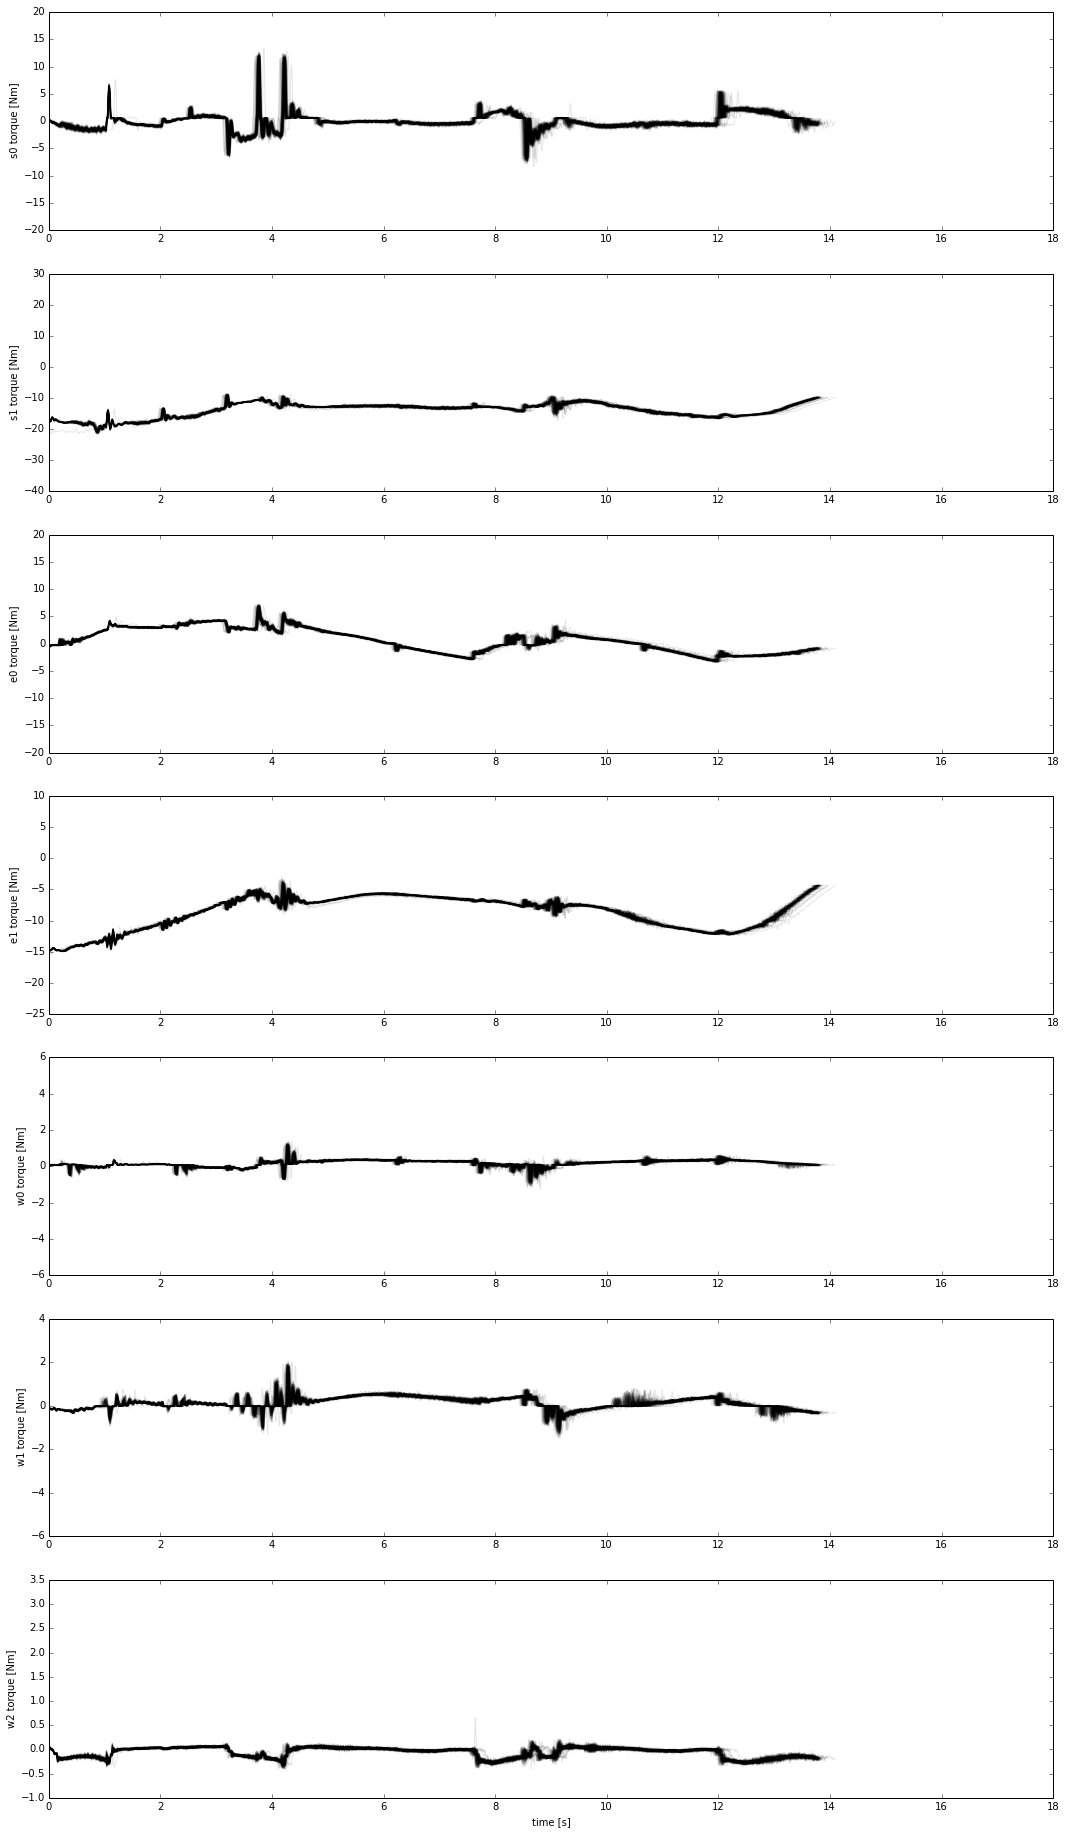
\includegraphics[width=.7\textwidth]{figs/no_anomaly3.png}
        \caption{100 trials of anomaly-free data.
            The seven rows correspond to seven joints of the left arm, ordered from proximal (s0) to distal (w2).
            The $y$-axis corresponds to torques in Nm, the $x$-axis to time in s.
            The 100 consecutive trials are overlaid in the figure.}
        \label{fig:noanomaly}
    \end{figure}
    
    The same plot for the anomalous data shows that it is much noisier than the ``normal'' data.
    This is illustrated in \cref{fig:controlbroke}.
    \begin{figure}
        \centering
        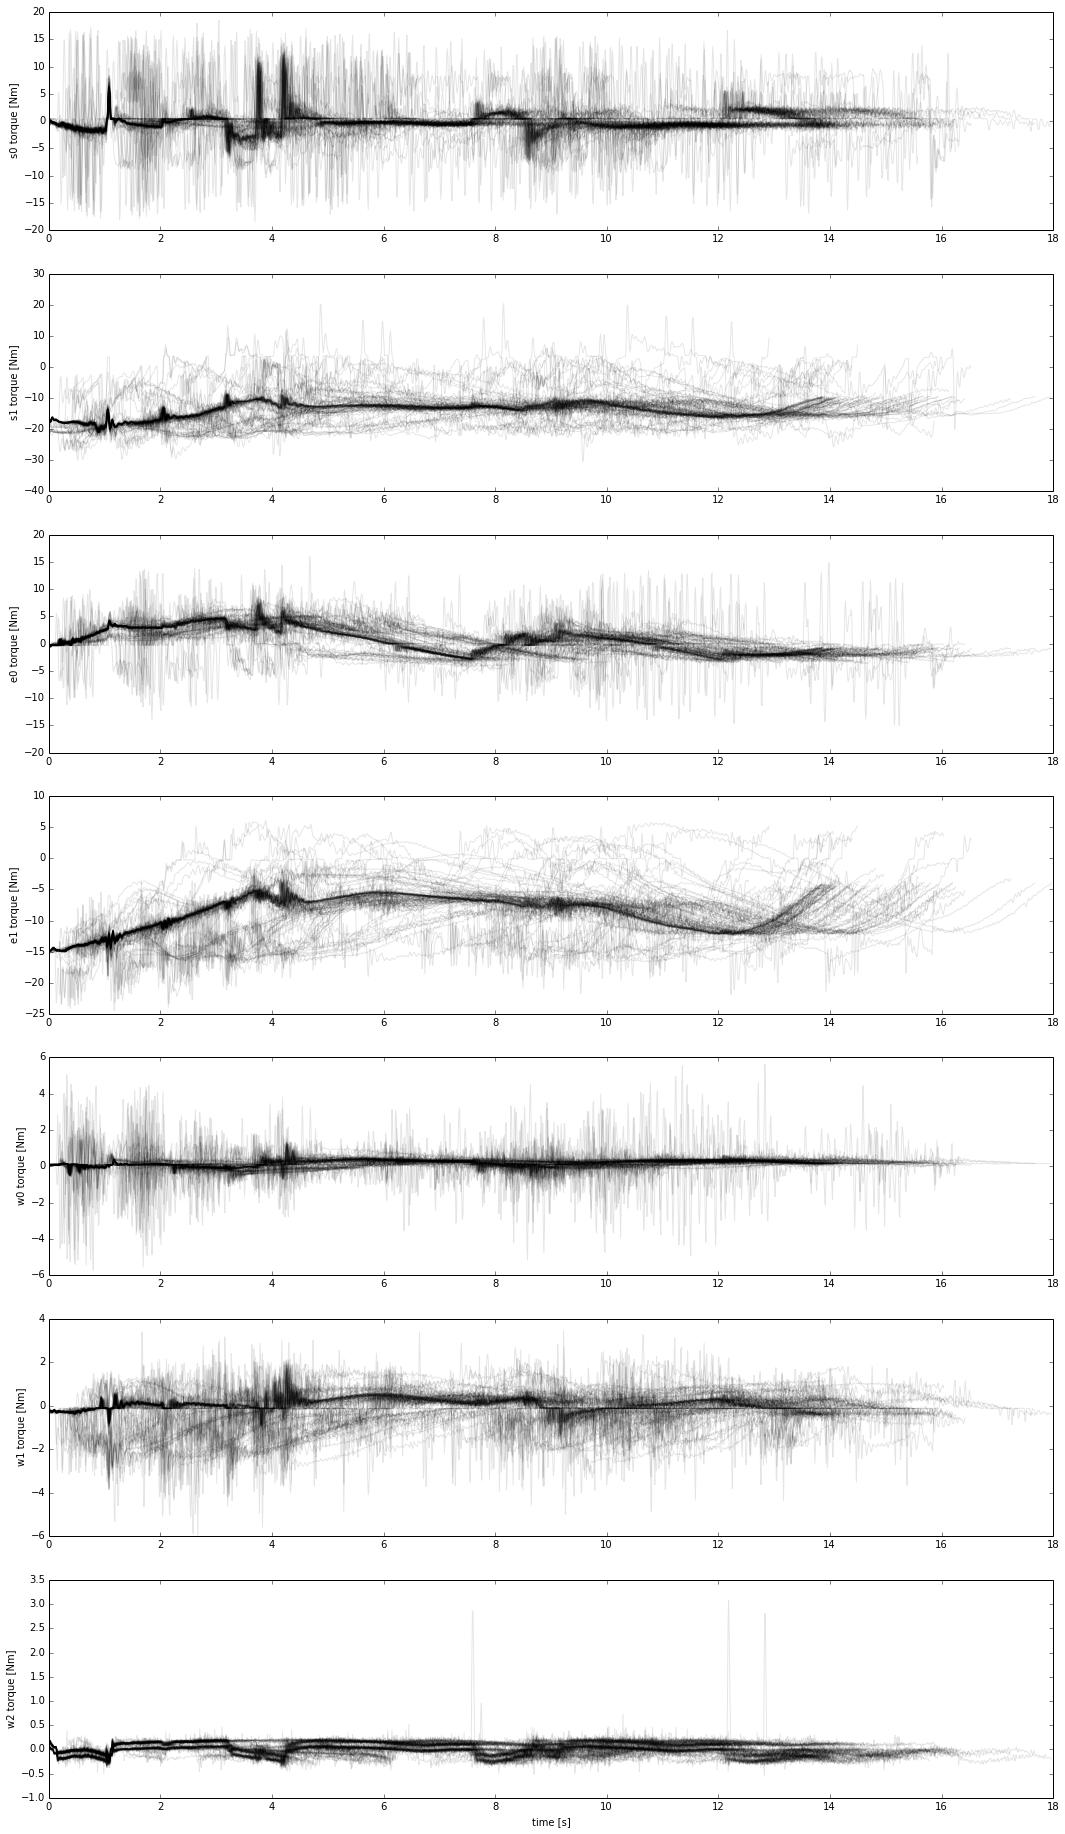
\includegraphics[width=.7\textwidth]{figs/controller_broke3.png}
        \caption{100 trials of anomalous data, where the proportional control parameter is modified.
            The seven rows correspond to seven joints of the left arm, ordered from proximal (s0) to distal (w2).
            The $y$-axis corresponds to torques in Nm, the $x$-axis to time in s.
            Anomalies were generated with probability $\Pi = 0.5$.
            The 100 consecutive trials are overlaid in the figure.}
        \label{fig:controlbroke}
    \end{figure}
    Let us now have a closer look at two particular anomalous trials.
    To see if and how the anomalous data differs from the ``normal'' data, we plot a single anomalous trial over the 100 anomaly-free trials in \cref{fig:noanomaly}.
    For the trial with index 12 in \texttt{201508071533with.h5} we obtain the plot in \cref{fig:anomaly12}.
    \begin{figure}
        \centering
        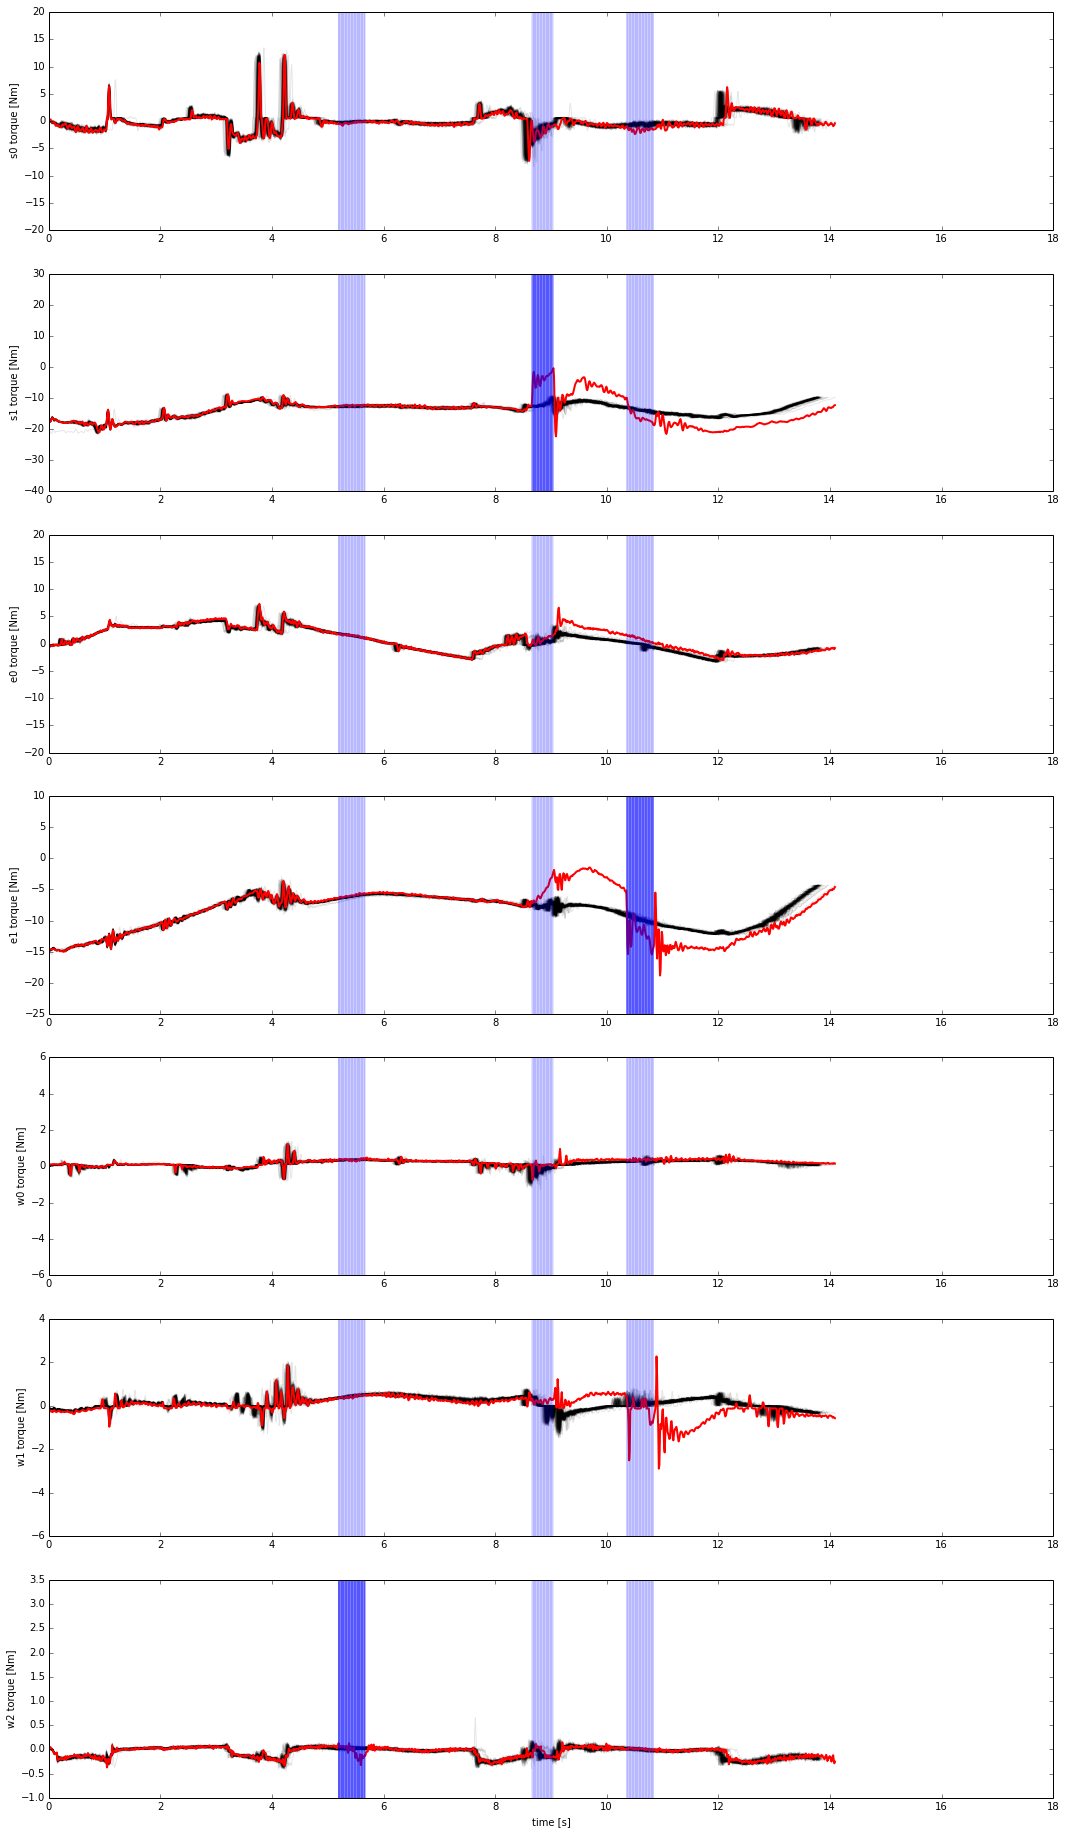
\includegraphics[width=.7\textwidth]{figs/anomaly12.png}
        \caption{Anomalous trial 12 (red) plotted over 100 overlaid, consecutive trials of ``normal'' data (black).
            The seven rows correspond to seven joints of the left arm, ordered from proximal (s0) to distal (w2).
            Blue shading indicates anomalous time steps as defined in \cref{sssec:anomaly}.
            Darker blue indicates the modified joint, lighter blue the response in the other joints due to the mechanical coupling.
            The $y$-axis corresponds to torques in Nm, the $x$-axis to time in s.}
        \label{fig:anomaly12}
    \end{figure}
    We see that deviations are clearly caused by the introduced anomaly and are mainly localized around the anomalous time steps.
    It appears valid to assume that it should be possible to learn a model that is able to detect the introduced anomalies. 
    
    For the trial with index 50 in \texttt{201508071533with.h5} (\cref{fig:anomaly50}) we see a different behavior.
    \begin{figure}
        \centering
        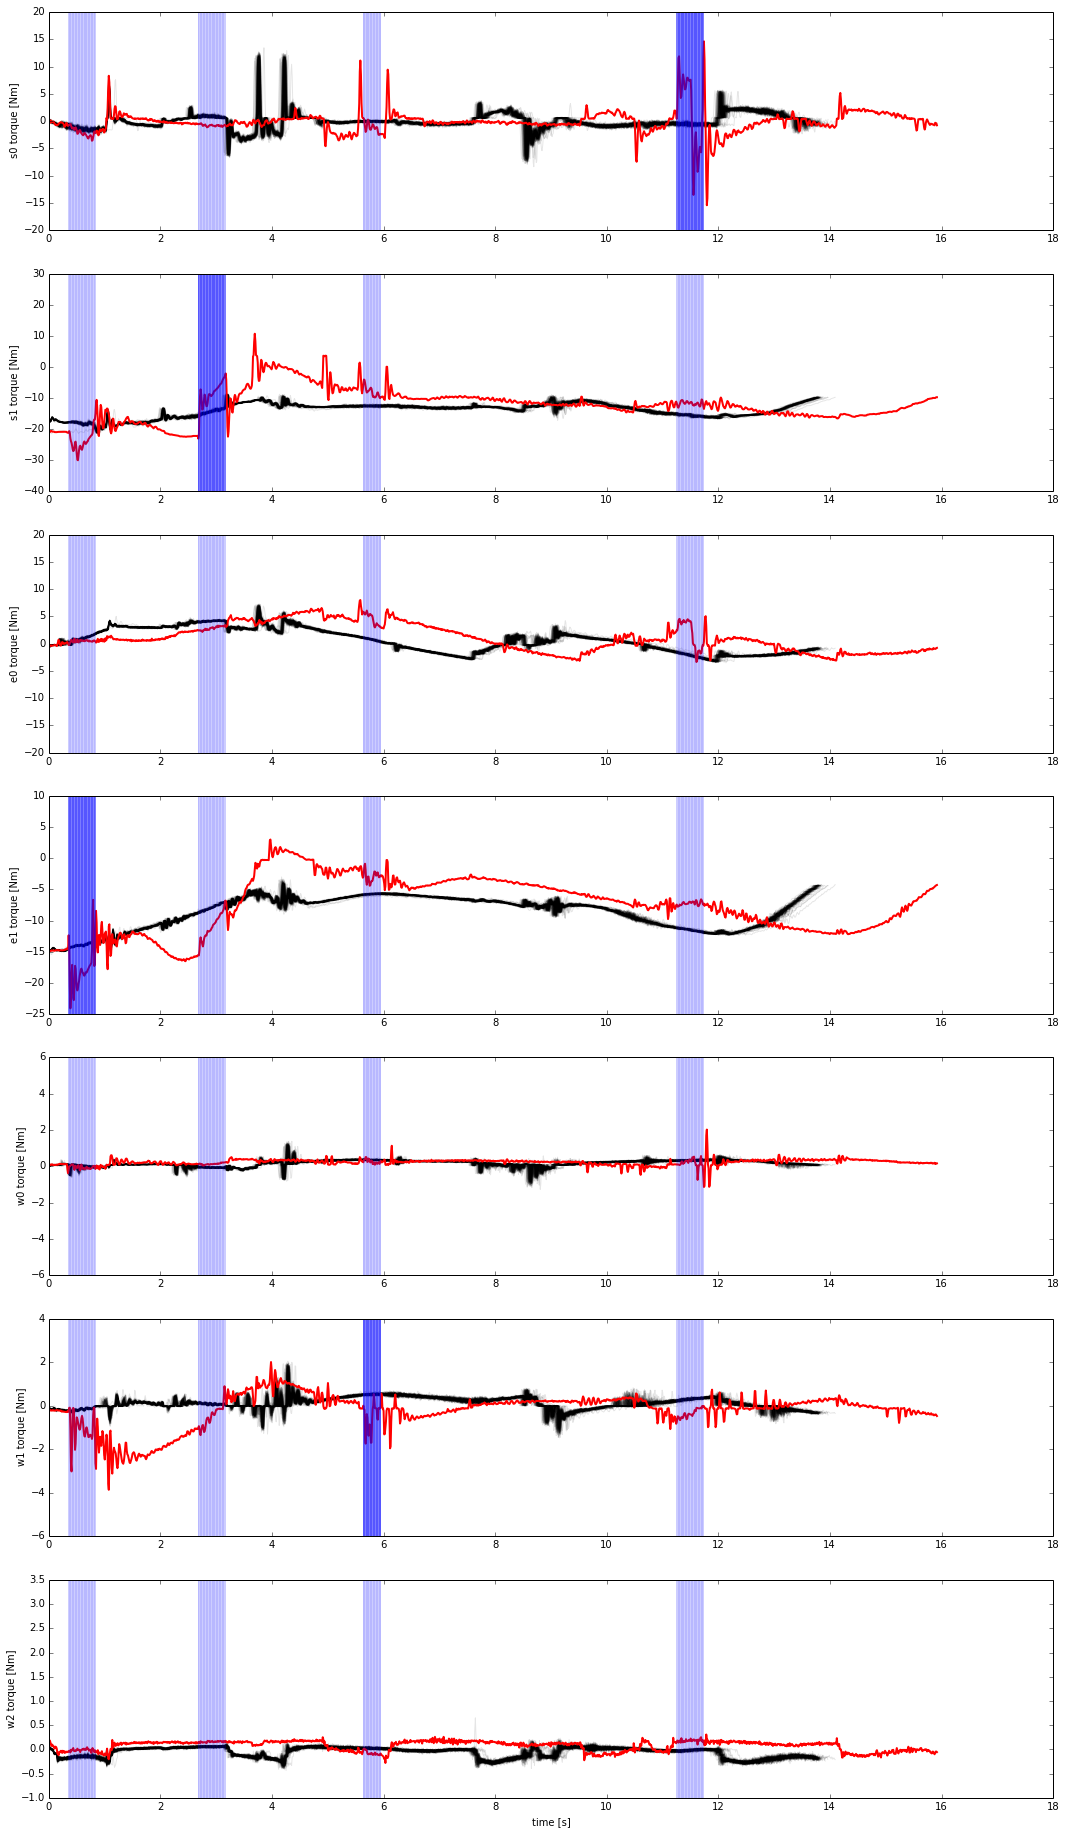
\includegraphics[width=.7\textwidth]{figs/anomaly50.png}
        \caption{Anomalous trial 50 (red) plotted over 100 overlaid, consecutive trials of ``normal'' data (black).
            The seven rows correspond to seven joints of the left arm, ordered from proximal (s0) to distal (w2).
            Blue shading indicates anomalous time steps as defined in \cref{sssec:anomaly}.
            Darker blue indicates the modified joint, lighter blue the response in the other joints due to the mechanical coupling.
            The $y$-axis corresponds to torques in Nm, the $x$-axis to time in s.}
        \label{fig:anomaly50}
    \end{figure}
    Additionally to the introduced anomalies there seems to be some scaling of the underlying trajectory.
    We can assume that this will make the detection of the introduced anomalies much harder.
    What is more, this sample shows the need to define how to handle the additional anomaly, i.e., the scaling effect, e.g.\ by normalization of the length of the time series data (which of course is not an option if we want to achieve (close-to) online detection of anomalies).


%\begin{thebibliography}{1}
%    
%    \bibitem{Steger2007} Steger, C., Ulrich, M.\ and Wiedemann, C.: \emph{Machine Vision Algorithms and Applications}. Wiley-VCH, Weinheim, 2007.
%    
%\end{thebibliography}


\appendix

\section{The \baxterrpc Framework}
\label{sec:baxterrpc}
    The \baxterrpc framework can be obtained from \url{https://bitbucket.org/lude-ma/baxterrpc}.
    It provides a JSON-RPC server implemented in Python that can be run on the Baxter research robot.
    This server has a selection of functions from Rethink Robotics' Baxter interface registered that can be called via remote procedure calls.

\section{The \baxterdotnet Framework}
\label{sec:baxterdotnet}
    The \baxterdotnet framework consists of two parts.
    The first part is the BaxterService, which can be obtained from \url{https://bitbucket.org/lude-ma/baxterservice}.
    It provides a C\# client connecting to the \baxterrpc server running on the Baxter research robot, thereby being a wrapper for Rethink Robotics' Baxter interface that can be called from a Windows machine.
    The second part is the DataAcquisition program, which can be obtained from \url{https://bitbucket.org/lude-ma/baxter}.
    It contains a C\# implementation of the experiment described in \cref{ssec:experiment}.
    
    It should be noted that the functionality described in this article is only a subset of the functionality implemented in the \baxterdotnet framework.
    The interested reader is referred to the extensive documentation of the libraries contained in the \baxterdotnet framework, namely \verb|baxterServer.dll|, \verb|baxterWrapper.dll| and \verb|control.dll|.
    
\end{document}
